% **************************************************
% Document Class Definition
% **************************************************
\documentclass[%
    paper=A4,               % paper size --> A4 is default in Germany
    twoside=true,           % onesite or twoside printing
    openright,              % doublepage cleaning ends up right side
    parskip=full,           % spacing value / method for paragraphs
    chapterprefix=true,     % prefix for chapter marks
    11pt,                   % font size
    headings=normal,        % size of headings
    bibliography=totoc,     % include bib in toc
    listof=totoc,           % include listof entries in toc
    titlepage=on,           % own page for each title page
    captions=tableabove,    % display table captions above the float env
    chapterprefix=false,    % do not display a prefix for chapters
    appendixprefix=false,   % but display a prefix for appendix chapter
    draft=false,            % value for draft version
]{scrreprt}%


% **************************************************
% Setup YOUR thesis document in this file !
% **************************************************
% !TEX root = main.tex


% **************************************************
% Files' Character Encoding
% **************************************************
\PassOptionsToPackage{utf8}{inputenc}
\usepackage{inputenc}


% **************************************************
% Information and Commands for Reuse
% **************************************************
\newcommand{\thesisTitle}{Advanced Ranking Sampling
	Strategies for Monocular Depth
	Estimation}
\newcommand{\thesisName}{Praneeth Balakrishna}
\newcommand{\thesisSubject}{Master’s Thesis}
\newcommand{\thesisDate}{December 10, 2021}
\newcommand{\thesisVersion}{My First Draft}

\newcommand{\thesisFirstReviewer}{Prof. Dr. Eyke H\"ullermeier}
\newcommand{\thesisFirstReviewerUniversity}{\protect{Paderborn University}}
\newcommand{\thesisFirstReviewerDepartment}{Department of Computer Science}

\newcommand{\thesisSecondReviewer}{Prof. Dr. Marco Platzner}
\newcommand{\thesisSecondReviewerUniversity}{\protect{Paderborn University}}
\newcommand{\thesisSecondReviewerDepartment}{Department of Computer Science}

\newcommand{\thesisFirstSupervisor}{Mr. Julian Lienen}
%\newcommand{\thesisSecondSupervisor}{John Smith}

\newcommand{\thesisUniversity}{}
\newcommand{\thesisUniversityDepartment}{Department of Computer Science}
\newcommand{\thesisUniversityInstitute}{Paderborn University}
\newcommand{\thesisUniversityGroup}{Intelligent Systems Group (ISG)}
\newcommand{\thesisUniversityCity}{Paderborn}
\newcommand{\thesisUniversityStreetAddress}{Pohlweg 51}
\newcommand{\thesisUniversityPostalCode}{33098}


% **************************************************
% Debug LaTeX Information
% **************************************************
%\listfiles


% **************************************************
% Load and Configure Packages
% **************************************************
\usepackage[english]{babel} % babel system, adjust the language of the content
\PassOptionsToPackage{% setup clean thesis style
    figuresep=colon,%
    hangfigurecaption=false,%
    hangsection=true,%
    hangsubsection=true,%
    sansserif=false,%
    configurelistings=true,%
    colorize=full,%
    colortheme=upbisg,%    
    % todo    to block the bib settings of the template
%    configurebiblatex=true,%
%    bibsys=biber,%
%    bibfile=bib-refs,%
%    bibstyle=alphabetic,%
%    bibsorting=nty,%
}{cleanthesis}
\usepackage{cleanthesis}

\usepackage{mathtools}

\hypersetup{% setup the hyperref-package options
    pdftitle={\thesisTitle},    %   - title (PDF meta)
    pdfsubject={\thesisSubject},%   - subject (PDF meta)
    pdfauthor={\thesisName},    %   - author (PDF meta)
    plainpages=false,           %   -
    colorlinks=false,           %   - colorize links?
    pdfborder={0 0 0},          %   -
    breaklinks=true,            %   - allow line break inside links
    bookmarksnumbered=true,     %
    bookmarksopen=true          %
}

% **************************************************
% Other Packages
% **************************************************
\usepackage{scrhack}
\usepackage{amsmath, amsfonts, amssymb}
\usepackage{placeins}
\usepackage{subcaption}
\usepackage{enumitem}
\usepackage{setspace}
\usepackage{cite}
\usepackage{graphicx, caption}
\usepackage{svg}
\usepackage{threeparttable}%
\usepackage{algorithmic}
\usepackage[linesnumbered,ruled,vlined]{algorithm2e}


% **************************************************
% Document CONTENT
% **************************************************
\begin{document}

% --------------------------
% rename document parts
% --------------------------
%\renewcaptionname{ngerman}{\figurename}{Abb.}
%\renewcaptionname{ngerman}{\tablename}{Tab.}
\renewcaptionname{english}{\figurename}{Fig.}
\renewcaptionname{english}{\tablename}{Tab.}

% --------------------------
% Front matter
% --------------------------
\pagenumbering{roman}			% roman page numbing (invisible for empty page style)
\pagestyle{empty}				% no header or footers
% !TEX root = ../main.tex
%
% ------------------------------------  --> cover title page
\begin{titlepage}
	\pdfbookmark[0]{Cover}{Cover}
	\flushright
	\hfill
	\vfill
	{\LARGE\thesisTitle \par}
	\rule[5pt]{\textwidth}{.4pt} \par
	{\Large\thesisName}
	\vfill
	\textit{\large\thesisDate} \\
	Version: \thesisVersion
\end{titlepage}


% ------------------------------------  --> main title page
\begin{titlepage}
	\pdfbookmark[0]{Titlepage}{Titlepage}
	\tgherosfont
	
	\begin{figure}
	\begin{minipage}[t]{8.5cm}		
	
\includegraphics[height=1.8cm]{gfx/upb_1E}\\
	\textsf{\small{\hspace*{1.3cm}Department of Electrical Engineering,\\
	\hspace*{1.3cm}Computer Science and Mathematics\\
%		\hspace*{1.3cm}Institute of Computer Science\\
		\hspace*{1.3cm}Warburger Straße 100 \\
		\hspace*{1.3cm}33098 Paderborn
		}}
	\end{minipage}
	\hfill
	\begin{minipage}[t]{4.7cm}
	
\includegraphics[height=1.8cm]{gfx/is-logo-klein}\\
	\textsf{%Institute of Computer Science\\
	\hspace*{0.1cm}\small{Intelligent Systems Group (ISG)}
	}
	\end{minipage}
	\end{figure}
	
	\centering
	%\textsf{\thesisUniversityDepartment} \\
	%\textsf{\thesisUniversityInstitute} \\
	%\textsf{\thesisUniversityGroup} \\

	\vfill
	{\large \thesisSubject} \\[5mm]
	{\LARGE \color{ctcolortitle}\textbf{\thesisTitle} \\[10mm]}
	{\Large \thesisName} \\

	\vfill
	\begin{minipage}[t]{.27\textwidth}
		\raggedleft
		\textit{1. Reviewer}
	\end{minipage}
	\hspace*{15pt}
	\begin{minipage}[t]{.65\textwidth}
		{\Large \thesisFirstReviewer} \\
	  	{\small \thesisFirstReviewerDepartment} \\[-1mm]
		{\small \thesisFirstReviewerUniversity}
	\end{minipage} \\[5mm]
	\begin{minipage}[t]{.27\textwidth}
		\raggedleft
		\textit{2. Reviewer}
	\end{minipage}
	\hspace*{15pt}
	\begin{minipage}[t]{.65\textwidth}
		{\Large \thesisSecondReviewer} \\
	  	{\small \thesisSecondReviewerDepartment} \\[-1mm]
		{\small \thesisSecondReviewerUniversity}
	\end{minipage} \\[10mm]
	\begin{minipage}[t]{.27\textwidth}
		\raggedleft
		\textit{Supervisors}
	\end{minipage}
	\hspace*{15pt}
	\begin{minipage}[t]{.65\textwidth}
		\thesisFirstSupervisor\ %and \thesisSecondSupervisor
	\end{minipage} \\[10mm]

	\thesisDate \\

\end{titlepage}


% ------------------------------------  --> lower title back for single page layout
\hfill
\vfill
{
	\small
	\textbf{\thesisName} \\
	\textit{\thesisTitle} \\
	\thesisSubject, \thesisDate \\
	Reviewers: \thesisFirstReviewer\ and \thesisSecondReviewer \\
	Supervisors: \thesisFirstSupervisor\ %and \thesisSecondSupervisor \\[1.5em]
	\textbf{\thesisUniversity} \\
	\textit{\thesisUniversityGroup} \\
	\thesisUniversityInstitute \\
	\thesisUniversityDepartment \\
	\thesisUniversityStreetAddress \\
	\thesisUniversityPostalCode\ and \thesisUniversityCity
}
		% INCLUDE: all titlepages
%\cleardoublepage
\pagestyle{plain}				% display just page numbers
% !TEX root = ../my-thesis.tex
%
\pdfbookmark[0]{Abstract}{Abstract}
\chapter*{Abstract  Todo}
\label{sec:abstract}
\vspace*{-10mm}

%\blindtext

\vspace*{20mm}

%{\usekomafont{chapter}Abstract (different language)}\label{sec:abstract-diff} \\

%\blindtext

\cleardoubleemptypage		% INCLUDE: the abstracts (english and german)
\cleardoublepage
%
% !TEX root = ../my-thesis.tex
%
\pdfbookmark[0]{Acknowledgement}{Acknowledgement}
\chapter*{Acknowledgement TODO}
\label{sec:acknowledgement}
\vspace*{-10mm}

%\Blindtext[2][2]
 % INCLUDE: acknowledgement
\cleardoublepage
%
\currentpdfbookmark{\contentsname}{toc}
\setcounter{tocdepth}{2}		% define depth of toc
\tableofcontents				% display table of contents
\cleardoublepage

% --------------------------
% Body matter
% --------------------------
\pagenumbering{arabic}			% arabic page numbering
\setcounter{page}{1}			% set page counter
\pagestyle{scrheadings} 	% fancy header and footer

% !TEX root = ../my-thesis.tex
%
\chapter{Introduction}
\label{sec:intro}

\cleanchapterquote{You can’t do better design with a computer, but you can speed up your work enormously.}{Wim Crouwel}{(Graphic designer and typographer)}



\section{Postcards: My Address}
\label{sec:intro:address}

\textbf{Praneeth Balakrishna} \\
Vogeliusweg 23D.2.5 \\
33100 Paderborn \\
Germany


\section{Motivation}
\label{sec:intro:motivation}

Depth estimation is a well studied problem in computer vision. It is an important step in the 3-D reconstruction of scenes and is crucial in fields like robot-vision and self driving cars. Monocular depth estimation aims to solve this problem using images obtained from a single camera.
Humans can easily infer depth from single images with sufficient samples learnt(how near and far objects appear) over the lifetime. In contrast, for a computer vision system, monocular depth estimation is an ill posed problem due to its inherent ambiguity in mapping RGB pixel values to depth.
\\\\
Typically, this is solved as a regression problem where the learning model learns to predict the metric depth map of the given RGB image. Such a depth map contains the metric depth of every pixel/segment within the image. Deep learning models, especially Convolutional Neural Networks(CNN) have achieved good success in learning such models, as demonstrated in \cite{eigen2014depth}. Such a technique requires training data which also contains a metric depth map which is obtained using much complex techniques such as methods utilizing sensors like Lidar and Kinect.\\
However, not all applications require exact metric depth prediction. Instead, prediction of an ordinal relation is sufficient in such cases, \textit{e.g.}, to detect occlusion boundaries in the image for an augmented reality application.  This also provides an opportunity for models to learn from pseudo depth data \cite{zoran2015learning,chen2016single}. Pseudo depth maps only provide relative depth information such as object A 'is closer' than object B or object B 'is closer' than object C, but does not quantify the distance between them. Furthermore, such an ordinal classification problem can be solved as a ranking problem \cite{liu2011learning}. \cite{xian2018monocular,xian2020structure} employ learning-to-rank methods on pairwise training samples, minimizing pairwise ranking loss in order to predict a dense pseudo-depth map. However, pairwise prediction leads to loss of information, particularly information about the transitivity of the order relation\cite{Lienen_2021_CVPR}. In order to overcome this issue, list-wise ranking was proposed \cite{cao2007learning}, where an arbitrary number of samples are chosen as a list and the model is trained to rank the samples in the order of their relative depth \cite{Lienen_2021_CVPR}. This is achieved by minimizing a permutation loss function which computes the inconsistency between the output ranking predicted by the model and the ground truth permutation. Such a model aims to solve a much complex ranking problem wherein the transitivity of all elements in the list of an arbitrary length is to be considered.
In the monocular depth estimation methods described in \cite{xian2018monocular,chen2016single,Lienen_2021_CVPR}, sampling methods utilized for training the model is predominantly random sampling of pairs or lists. Random sampling leads to two potential issues. Firstly, it leads to imbalanced ordinal relations\cite{xian2018monocular} and secondly, it misses out the fact that certain pixels in the image provide better depth cues than others. 
\\\\
In an attempt to further improve the performance of list-wise learning-to-rank method for monocular depth estimation \cite{Lienen_2021_CVPR}, two potential methods are explored in this thesis. 
Firstly, an informativeness score is computed over the training data by making use of the visual depth cues in the images and the learning model is trained on highly informative samples that provide better cues for depth estimation. 
Secondly, a query strategy on a partially trained model is developed such that, the model queries samples from the unlabeled training data about which it is most uncertain with respect to relative depth prediction. Thereby, choosing to learn from training samples that it is most uncertain of. Such a technique lies in the realm of active learning\cite{settles2009active} where the current model hypothesis is utilized within the query selection process for labelling samples for further training.




\section{Problem Statement}

The fundamental goal of the thesis is to solve the monocular depth estimation (of pixels) problem as a learning-to-rank task. However, the challenge is to achieve this by weakly supervised training data where the learning model does not learn from accurate metric depth, but instead learn from relative-depth training data. The methods described in Sec Todo !!!!! achieve laudable results in solving such a problem. The focus here is to improve those methods in order to achieve better results.

\subsection{Improved sampling strategy}
In methods \cite{xian2018monocular, chen2016single, Lienen_2021_CVPR}, the learning models are trained with samples(pairs or lists) that are randomly sampled from the training images. There are certain aspects of the image, like depth-edges, texture, occlusion, etc. that provide depth cues and random sampling misses out on entirely utilizing such information and hence, the model learns mostly from less informative samples.
Therefore, the aim is to propose an information measurement score on the training samples and develop a superior sampling strategy such that informative samples are more likely picked during training.

\subsection{Active learning}
Active learning is a case of machine learning where the learning algorithm chooses the data on which it learns \cite{settles2009active}. The model poses queries on unlabeled data to an oracle(eg. a human annotator), for the label. By this method, the learning model can learn effectively on fewer number of training samples.\\
Therefore, the second aim of the thesis is to develop an active learning algorithm to query uncertain samples for labeling, during prediction. Additionally, an oracle which can label the queried samples is to be formulated.   

Finally, an analysis of the performance improvement with both the above techniques is to be conducted in comparison to the earlier methods.  



\section{Results : TODO}
\label{sec:intro:results}

%\Blindtext[1][2]

\section{Thesis Structure}
\label{sec:intro:structure}
\textbf{Chapter \ref{sec:fundamentals}} \\[0.2em]
Chapter \ref{sec:fundamentals}  gives an overview of most of the necessary topics and various terminologies that are needed to understand the chapters that follow. It begins with describing the fundamental concepts of computer vision and also traces the various methods in which features can be extracted from images. This is followed by the topic Deep Learning which has resulted in a revolution in the field of artificial intelligence. Popular deep learning techniques pertaining to monocular depth estimation are discussed here. A brief description of the programming tools and frameworks needed to realize such models is also provided.

\textbf{Chapter \ref{sec:related}} \\[0.2em]


\textbf{Chapter \ref{sec:system}} \\[0.2em]


\textbf{Chapter \ref{sec:concepts}} \\[0.2em]


\textbf{Chapter \ref{sec:concepts}} \\[0.2em]


\textbf{Chapter \ref{sec:conclusion}} \\[0.2em]

   % INCLUDE: introduction




\chapter{Fundamentals}
\label{sec:fundamentals}

\cleanchapterquote{A picture is worth a thousand words. An interface is worth a thousand pictures.}{Ben Shneiderman}{(Professor for Computer Science)}


\section{Computer Vision}
\label{sec:fundamentals:sec1}

Computer vision is a field of artificial intelligence which aims to develop techniques that aid machines/computers to see and make meaningful inferences out of the content present in digital images.
Computer vision is the core idea in various applications namely Autonomous driving: for lane and pedestrian detection, in Healthcare: for medical imaging and cancer/tumour detection, in Manufacturing: for defect inspection, OCR/bar-code reading and preventive maintenance and in Agriculture: for crop yield monitoring, livestock health monitoring and crop disease detection.

Although the applications of computer vision is manifold, there exists a sequence of distinct steps to process and analyze images. Such a process can be termed as the vision pipeline.\cite{WEB:manning}. The following figure \ref{fig:fundamentals:example1} illustrates a typical vision pipeline followed in computer vision applications.

% \begin{figure}[!h]
% 	\centering
% 	\input{imgs/cvp.pdf}
% \end{figure}
\begin{figure}[h]
	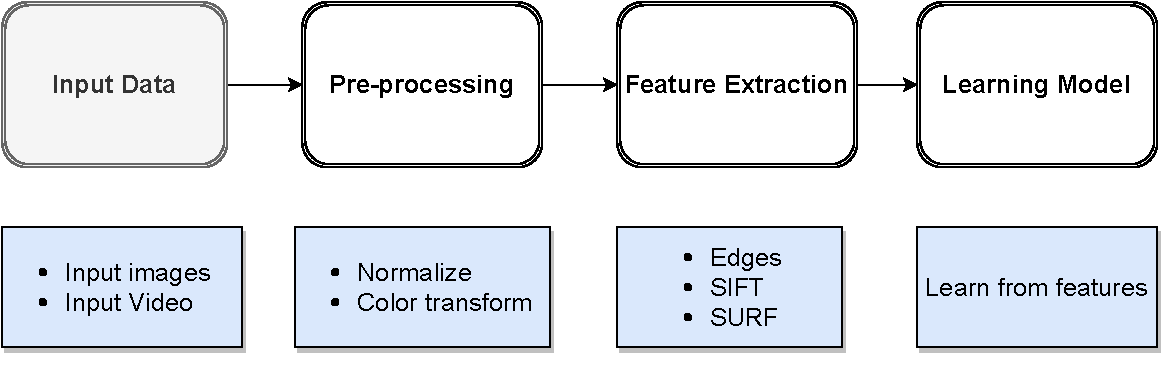
\includegraphics[width=\textwidth]{content/imgs/cv-pipeline.drawio.pdf}
	\caption{Computer vision pipeline}
	\label{fig:fundamentals:example1}
\end{figure}

\subsection{Input Data}
Computer vision applications typically deal with image or video data. A simple grayscale image can be represented as a 2-Dimensional function $F(x,y)$ over $x$ and $y$. where $F(x,y)$ is the intensity of the pixel at position $(x,y)$\\
In colour images, a third dimension is added which represents the intensities of different colour channels in the image. A typical color model is the RGB color model which stands for "Red, Green and Blue". A colour image in RGB format would be:
\begin{align*}
    \text{RGB image} = F(x,y) = [Red(x,y), Green(x,y), Blue(x,y)]
\end{align*}
which consists of three channels $Red(x,y), Green(x,y), Blue(x,y)$ each of dimensions $m$x$n$. Each channel represents the intensity map of the particular colour at every position $(x,y)$ in the image.\\
Each Color (that is a triplet of values (R, G, B)) has a depth of 24 bits (3 image planes times the number of bits per plane).
This results in $(2)^{24}$ different colour\cite{gonzalez2002digital}.


\subsection{Image Preprocessing}
The images acquired usually come from various sources and are often not clean. There could be a varied amount of noise, illumination differences and different contrasts. In order to feed them to a machine learning application, they need to be standardized and cleaned up \cite{WEB:manning}. It is nearly impossible to clean up each sample individually. Therefore a general procedure is followed to achieve this task.

%\begin{enumerate*}[label=\arabic*)]
%	\item Convert images to grayscale to reduce complexity: Certain applications like edge detection and depth estimation do not require information from all the three channels(in the case of RGB) in order to perform. In such cases it is useful to remove unwanted information from the image to reduce space and computational complexity \cite{WEB:manning}
%	
%	\item sdf 
%	
%\end{enumerate*}

\begin{enumerate}
	\item \textbf{Convert images to grayscale to reduce complexity:} Certain applications like edge detection and depth estimation do not require information from all the three channels(in the case of RGB) in order to perform. In such cases it is useful to remove unwanted information from the image to reduce space and computational complexity \cite{WEB:manning}
	
	\item \textbf{Standardize images:} Algorithms involving learning models have a fixed input shape requirement. In order to satisfy this requirement, the images from various sources must be scaled and reshaped to match the input dimensions of the learning models \cite{WEB:manning} .
	
	\item \textbf{Data augmentation:} Data augmentation is a method to increase the amount of training samples by making copies of the existing samples but however with slight changes in either orientation, translation, color intensity, etc. This exposes the learning model to a wider range of variations in the images and hence acts as a regularizer \cite{WEB:manning}.
	
\end{enumerate}


\subsection{Feature Extraction}
Machine learning models perform only as good as the features that they are trained on. Therefore, identifying and quantifying good quality features is crucial. Feature extraction consists of two steps: Feature detection and feature description \cite{gonzalez2002digital}. Feature detection refers to finding useful features in the image where as feature description assigns quantitative attributes to to the detected features \cite{gonzalez2002digital}.
Traditional computer vision problems relied heavily on manual feature engineering and selection. Such a task relied on the domain knowledge of the respective domain experts. The extracted features are then used to train learning models to realize a computer vision objective such as object detection, etc. 
Some examples of feature sets are:
\begin{itemize}
	\item Histogram of Oriented Gradients
	\item Haar Cascades
	\item Scale Invariant Feature Transform (SIFT)
	\item Speeded Up Robust Feature (SURF)
\end{itemize}

A detailed description of machine learning models used in computer vision applications are provided in the next section.


\section{Deep Learning}
\label{sec:fundamentals:deeplearning}


The inception of Machine learning had a primary objective of solving the problems faced by systems that rely on hard-coded information in order to function. Hence Machine learning emerged as a subset of Artificial Intelligence(AI), giving systems the ability to acquire their own knowledge by extracting information patterns from data without being explicitly programmed. However the performance of simple machine learning algorithms depends heavily on the representation of data that they are trained on \cite{Goodfellow-et-al-2016}. These representations of the raw data are called features and machine learning algorithms only learn to map such features to an output. 
For many tasks however, identifying what features are to be extracted is a difficult task by itself. For example, suppose we need a system to identify human faces in images. Here, one would like to use the presence of eyes as features. Unfortunately, it is very difficult to describe what eyes exactly look like in terms of image pixel values. Therefore, identifying and extracting features is a challenging task in most non trivial cases.

Deep Learning solves this central problem in representation learning by introducing representations that are expressed in terms of other, simpler representations \cite{Goodfellow-et-al-2016}. Deep learning technique uses abstract elements called neural networks to learn the representations of data and also models such high level abstractions in data using multiple non-linear transforms. Figure \ref{fig:deep learning model} demonstrates how a deep learning model can represent an image as multiple abstract feature representations like contours and object parts which are in turn represented as edges at a lower abstraction.
In this manner, deep learning class of algorithms eliminate the need of manual feature engineering by employing techniques which inherently perform hierarchical feature extraction from the given data.
It is based on cascaded layers of non-linear processing units, where the output of one layer is provided as an input to the next layer. The initial
layers are responsible for extracting the lower level features from the data. This learned information is then
fed to the next layer, which attempts to learn the higher-level features to form a hierarchical representation.
These algorithms can operate in both supervised as well as the unsupervised manner and therefore can be
used in applications like pattern recognition, classification tasks, etc.


\begin{figure}[t]
	%\vspace*{-2.1 in}
	\centering
	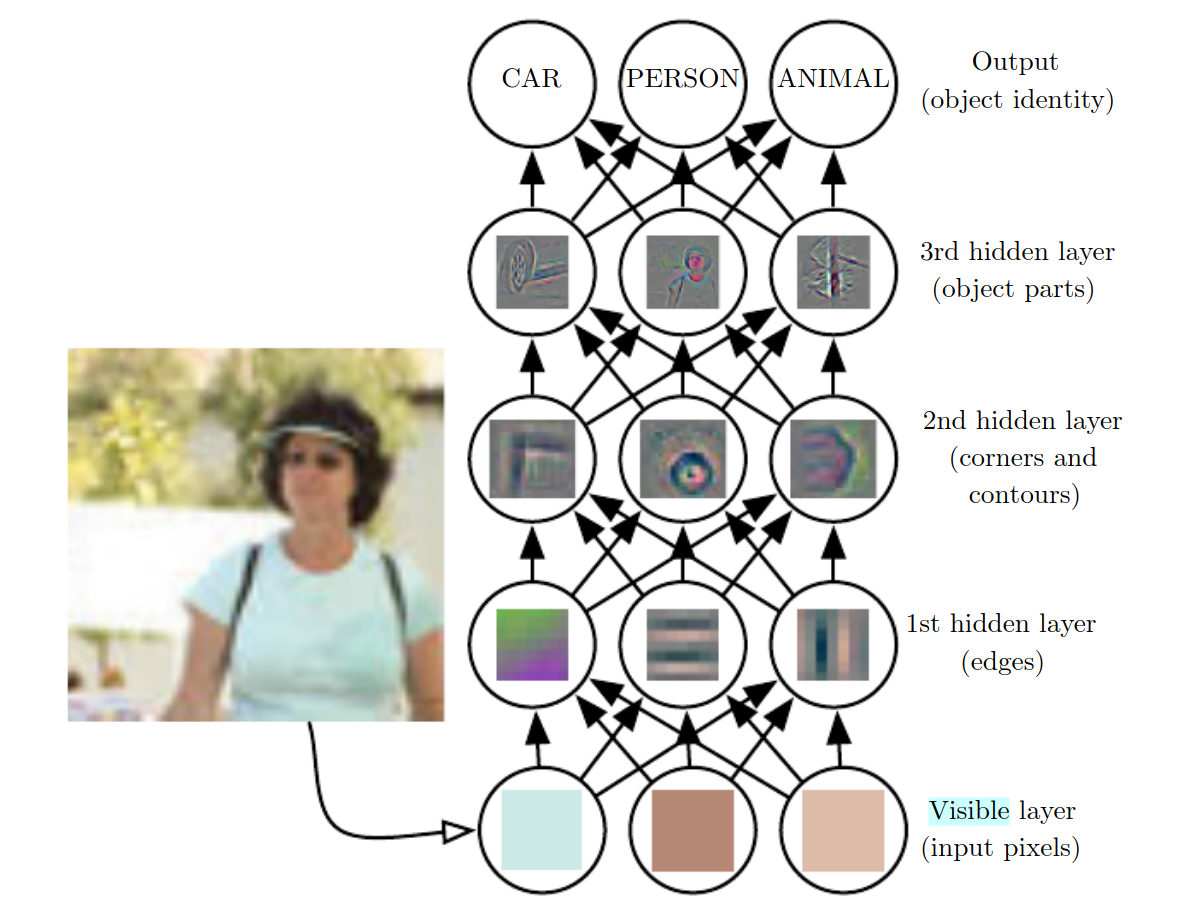
\includegraphics[width=\textwidth]{content/imgs/deep_learning_feature}
	\caption{Illustration of deep learning model. Source: \cite{Goodfellow-et-al-2016}}
	\label{fig:deep learning model}
\end{figure}



\begin{figure}[h]
	%\vspace*{-2.1 in}
	\centering
	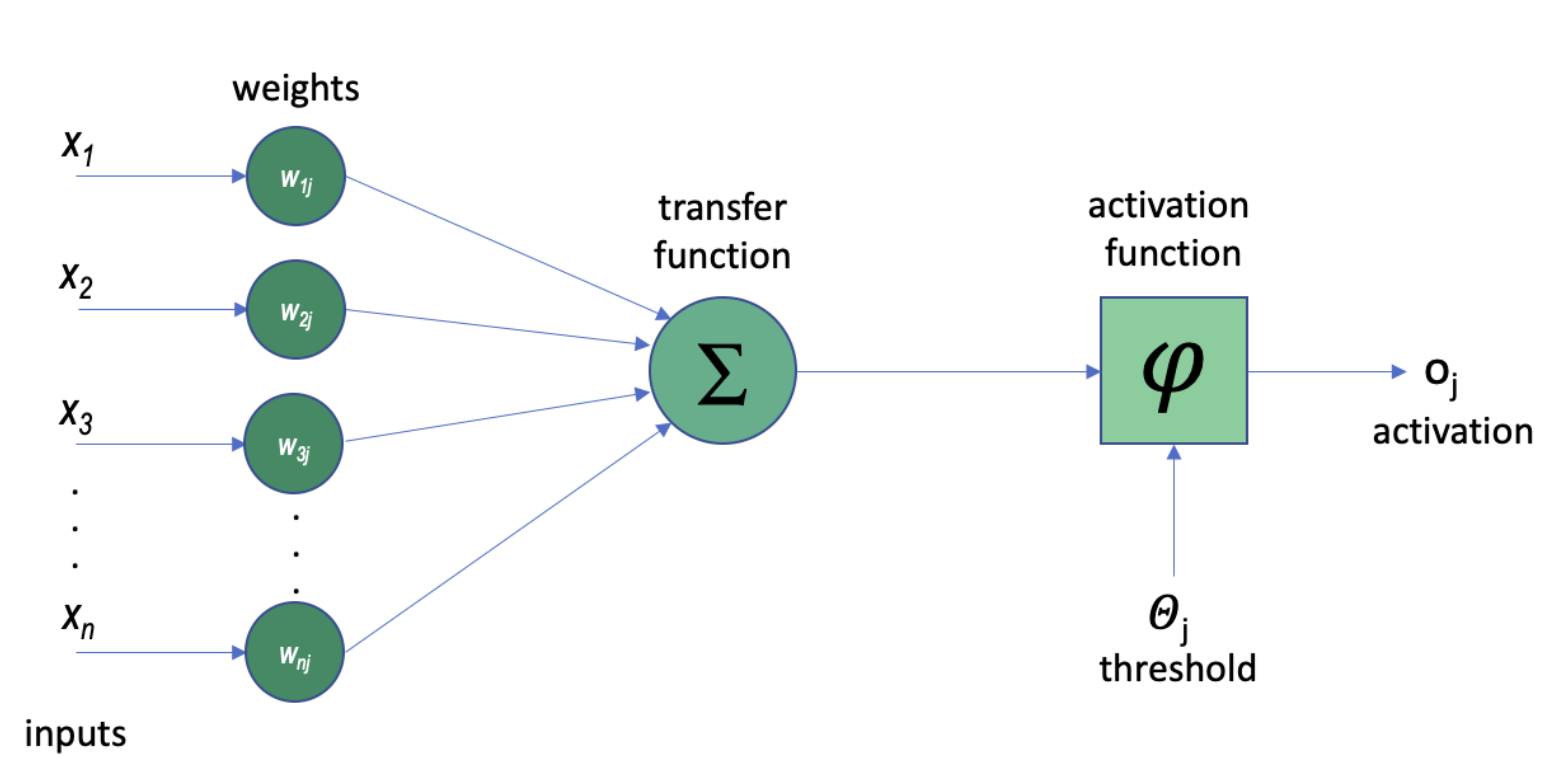
\includegraphics[width=\textwidth]{content/imgs/neuron}
	\caption{A single node of a neural network}
	\label{fig: neuron}
\end{figure}

The quintessential example of a deep learning model is the Multilayer Perceptron (MLP) \cite{Goodfellow-et-al-2016}. A multilayer perceptron is a mathematical function with certain non-linearity which maps a set of inputs to output values. Each application of such a function can be thought of as providing a new representation of the input data. Deep learning further breaks the complicated task of generating representations into series of nested mappings, each described by a different layer of the model \cite{Goodfellow-et-al-2016}. As shown in Figure \ref{fig:deep learning model}, the input data consisting of observable variables are presented at the `Visible layer'. This is followed by a series of `hidden layers' which form abstract representations from the input. Each layer in the network is comprised of multiple nodes which perform the computations. Each node or neuron performs a linear combination of the set of inputs at its level and a set of weights and passes it through an activation function. The weights signify the relevance of the input component it acts upon. The sum-of-products of the input and weights are then passed through an activation function, which determines the output of the particular node. The activation function has an optional threshold value. If the sum-of-products is greater than the threshold, the node produces an output and is said to be \textit{activated}. Figure \ref{fig: neuron} summarizes the operations in a single node/neuron.
Mathematically such an operation for the output of the $j$'th node at the $i$'th layer can be describes as:
\begin{align*}
	 o_j = \mathlarger \varphi \left( \sum X_i \cdot W_{ij} , \Theta_j \right) 
\end{align*}


Training a neural network essentially seeks to make the neural network learn the data representation behind the given raw input such that a predefined application specific cost function is minimized. This means that neural networks are trained using iterative, gradient-based optimizers that merely drives the cost function to a very low value \cite{Goodfellow-et-al-2016}. Variants of gradient descent and backpropagation are the crucial steps behind such iterative cost reduction technique used in deep learning. The derivative of the cost computed for a given prediction is computed with respect to each of the trainable parameters (weights) and subsequently updated in the direction of the negative gradient in an attempt to reduce the cost value. Using such an iterative optimization approach, neural networks are capable of learning any arbitrary function that maps the input to a suitable output.

In order to formally describe a deep neural network, it is essential to understand the following terms:

\begin{itemize}
	\item \textbf{Number of layers:} The number of layers in a deep learning model determines the depth of the model. It is a model architecture choice and purely depends on the complexity of the task at hand. A higher number of layers result in a more complex model which might cause problems like over-fitting and vanishing gradients. On the other hand, having very less number of layers results in a very simple model which might not even be able to learn the underlying representations in the data. This phenomenon leads to a problem called under-fitting. 
	
	\item \textbf{Cost Function:} The cost function is the criterion for optimization in all deep learning techniques. The cost function for deep neural networks is more or less similar to that of simpler parametric models such as linear models \cite{Goodfellow-et-al-2016}. In most cases the parametric model defines a distribution $p(y|x; \theta)$ where $y$ is the prediction, $x$ is the input and $\theta$ is the model parameter. In such cases the principle of maximum likelihood can be used and the negative likelihood can be used as the cost function. A classic example is the binary cross entropy loss used in binary classification tasks.
	
	\item \textbf{Activation function:} Popular activation functions used in deep learning are ReLU, sigmoid and tanh functions. In instances where a real number of any value is desired as an output, linear activation is used. The choice of activation function depends on the task and size of the network. However, sigmoid and tanh activation functions display the vanishing gradient problem for extreme values of their inputs. This factor must be considered while deciding for activation functions.
	
	\item \textbf{Optimizer:} Optimizers are algorithms to  iteratively minimize the cost function by altering the model parameters in order to improve the accuracy of the model. Therefore the choice of an optimizer is crucial in order to converge faster and avoid unfavorable local minima.
	Optimizers are typically gradient based techniques. Popular choices include Adam, Stochastic Gradient Descent(SGD) and RMSProp.
	
	\item \textbf{Learning rate:} The learning rate determines the size of the step taken in the direction of the optima in optimization algorithms. The choice of the learning rate determines the speed of convergence and the final optimum reached. A very low learning rate may make the training process very slow and hence takes a long time to converge. At the same time, a higher learning rate may cause the optimizer to overshoot the desired minima. Therefore, a balanced choice is to keep it adaptive, such that a higher learning rate is used in the beginning and subsequently decays over the training process.
	
	\item \textbf{Regularization:} Deep learning models are complex models with even millions of parameters in certain cases. This gives the model an enormous amount of flexibility to fit the training data. At times this can lead to overfitting to the training data. Hence regularization is essential to produce better generalization of the model. In L1 and L2 regularization, an additional regularization term is added to the cost function that penalizes large weights. However, Dropout regularization is the most popular technique for deep learning models. In dropout, at every training step each node has a probability $p$ of being turned off. The network learns accordingly, adapting to this change, thus reducing the chances of overfitting.
	
	\item \textbf{Epochs:} An epoch signifies one complete pass of the training data during the learning process. If the number of epochs is too large, it may cause the model to overfit to the data and may result in poor generalization on the test data. Whereas, if the number of epochs is too small, the model may not be able to learn the representations completely and may result in under-fitting. 
\end{itemize}


\section{Software Tools}
\label{sec:fundamentals:sw-tools}

This section briefly describes some of the most necessary software tools and frameworks used in realizing a deep learning based monocular depth estimation system for the thesis. 

\subsection{Python programming language}
Python is the world's fastest growing and popular programming language not just among software engineers and also among mathematicians, data analysts, scientists and accountants. Surveys like \cite{businessoverbroadway.com} \cite{rowe_2018} done worldwide also indicate that python is the most commonly used programming language for machine learning and data analysis. People from different disciplines use python for variety of different tasks such as data analysis and visualization, machine learning models and other automation.

\textit{Python}, which was originally developed in the late 1980's is an object oriented, high-level general purpose programming language \cite{van2007python}. It provides a wide array of built-in data structures and abstract data types which eases application development. One of the distinguishing factors of python is that it is an interpreted language, meaning it does not have a compilation step. This feature along with modularity and simple syntax makes debugging simpler, thus reducing development time through increased efficiency.

Artificial intelligence and machine learning has penetrated into most applications in today's world. Python has become the go-to language for machine learning and deep learning applications. Python comes with a myriad amount of libraries and frameworks that make coding easy. This also saves a significant amount of time. Python is an open-source programming language and enjoys excellent support from many resources and quality documentation along with a large and active community. Where speed is a concern, it provides alternatives like Cython, which is capable of producing performances similar to the C programming language. Also, being popular for the data analysis related tasks, Python provides very efficient interfaces to all major commercial as well as open-source databases. All these features allow Python to outshine in the field of data science compared to traditional languages like C++ and Java.


\subsection{Machine Learning Frameworks: TensorFlow}
TensorFlow \cite{abadi2016tensorflow} is a computation library developed by Google which has become very popular among the machine learning community. Though it was originally developed for numerical computation, it proves to be useful for deep learning applications too.
The fundamental data structure used in TensorFlow are multidimensional arrays called tensors. Each computation is represented graphically as a data flow graph \cite{tensorflow_2019} where each node in the graph represents a mathematical operation. 

Some of the key features of tensor-flow are as follows:
\begin{itemize}
	\item Though python is the preferred language for developing applications in TensorFlow, most of the underlying implementation is done in C++ and CUDA.
	
	\item TensorFlow provides comprehensive GPU support. This is crucial for training deep learning models faster and also facilitates training on distributed clusters.
	
	\item In contrast to sequential programming, a static computation graph consisting of nodes and edges is created and the graphs are executed in the form of sessions.
	
	\item \textit{tf.data} facilitates building of data pipelines efficiently including data pre-processing.
	
	\item Keras integrates tightly with TensorFlow \cite{tensorflow_2019}. This offers a variety of high-level API's which can be used to build complex models on top of low-level TensorFlow functions.   
	
\end{itemize}
 




\textbf{ todo : Additional buffer for more stuff if needed.}



   % Include: fundamentals
% !TEX root = ../my-thesis.tex
%
\chapter{Related Work}
\label{sec:related}

\cleanchapterquote{A picture is worth a thousand words. An interface is worth a thousand pictures.}{Ben Shneiderman}{(Professor for Computer Science)}



\section{Related Work Section 1}
\label{sec:related:sec1}



\section{Related Work Section 2}
\label{sec:related:sec2}



\section{Related Work Section 3}
\label{sec:related:sec3}



\section{Conclusion}
\label{sec:related:conclusion}


   % INCLUDE: related work
% !TEX root = ../my-thesis.tex
%
\chapter{System}
\label{sec:system}

\cleanchapterquote{Innovation distinguishes between a leader and a follower.}{Steve Jobs}{(CEO Apple Inc.)}



\section{System Section 1}
\label{sec:system:sec1}



\begin{figure}[htb]
	
\includegraphics[width=\textwidth]{gfx/Clean-Thesis-Figure}
	\caption{Figure example: \textit{(a)} example part one, \textit{(c)} example part two; \textit{(c)} example part three}
	\label{fig:system:example1}
\end{figure}



\section{System Section 2}
\label{sec:system:sec2}



\begin{figure}[htb]
	
\includegraphics[width=\textwidth]{gfx/Clean-Thesis-Figure}
	\caption{Another Figure example: \textit{(a)} example part one, \textit{(c)} example part two; \textit{(c)} example part three}
	\label{fig:system:example2}
\end{figure}



\section{System Section 3}
\label{sec:system:sec3}



\section{Conclusion}
\label{sec:system:conclusion}


         % INCLUDE: system
% !TEX root = ../my-thesis.tex
%
\chapter{Concepts: This text is here to test a very long title, to simulate the line break behavior, to show that an extremely long tilte also works}
\label{sec:concepts}

\cleanchapterquote{Users do not care about what is inside the box, as long as the box does what they need done.}{Jef Raskin}{about Human Computer Interfaces}



\section{Concepts Section 1}
\label{sec:concepts:sec1}



\section{Concepts Section 2}
\label{sec:concepts:sec2}



\section{Concepts Section 3}
\label{sec:concepts:sec3}



\section{Conclusion}
\label{sec:concepts:conclusion}


       % INCLUDE: concepts
% !TEX root = ../my-thesis.tex
%
\chapter{Conclusion}
\label{sec:conclusion}



\section{System Section 1}
\label{sec:conclusion:sec1}



\section{System Section 2}
\label{sec:conclusion:sec2}



\section{Future Work}
\label{sec:conclusion:future}


     % INCLUDE: conclusion

% --------------------------
% Back matter
% --------------------------
\appendix\cleardoublepage
% !TEX root = ../my-thesis.tex
%
\chapter{Example Appendix}
\label{sec:appendix}





\section{Appendix Section 1}
\label{sec:appendix:sec1}



\begin{table}[h]
	\begin{tabularx}{\textwidth}{X | X | X}
		%\hline
		Alpha		& Beta			& Gamma			\\ \hline
		0			& 1				& 2				\\ \hline
		3			& 4				& 5				\\ %\hline
	\end{tabularx}
	\label{tab:table1}
	\caption{This is a caption text.}
\end{table}

\section{Appendix Section 2}
\label{sec:appendix:sec2}



\begin{table}[h]
	\begin{tabularx}{\textwidth}{X | X | X}
		%\hline
		Alpha		& Beta			& Gamma			\\ \hline
		0			& 1				& 2				\\ \hline
		3			& 4				& 5				\\ %\hline
	\end{tabularx}
	\label{tab:table2}
	\caption{This is a caption text.}
\end{table}


       % INCLUDE: appendix
%

% todo  to block the bib of orig template
%{%
%\setstretch{1.1}
%\renewcommand{\bibfont}{\normalfont\small}
%\setlength{\biblabelsep}{0pt}
%\setlength{\bibitemsep}{0.5\baselineskip plus 0.5\baselineskip}
%\printbibliography[nottype=online]
%\newrefcontext[labelprefix={@}]
%\printbibliography[heading=subbibliography,title={Webpages},type=online]
%}
\bibliography{bib-refs}
\bibliographystyle{myalphadin}

\cleardoublepage

\listoffigures
\cleardoublepage

\listoftables
\cleardoublepage

% !TEX root = ../my-thesis.tex
%
\pagestyle{empty}
\hfill
\vfill
\pdfbookmark[0]{Colophon}{Colophon}
\section*{Colophon}

This thesis was typeset with \LaTeXe.
It uses the \textit{Clean Thesis} style developed by Ricardo Langner.
The design of the \textit{Clean Thesis} style is inspired by user guide documents from Apple Inc.

Download the \textit{Clean Thesis} style at \url{http://cleanthesis.der-ric.de/}.

\cleardoublepage

% !TEX root = ../my-thesis.tex
%
%************************************************
% Declaration
%************************************************
\pdfbookmark[0]{Declaration}{Declaration}
\chapter*{Declaration}
\label{sec:declaration}
\thispagestyle{empty}

You can put your declaration here, to declare that you have completed your work solely and only with the help of the references you mentioned.

\bigskip

\noindent\textit{\thesisUniversityCity, \thesisDate}

\smallskip

\begin{flushright}
	\begin{minipage}{5cm}
		\rule{\textwidth}{1pt}
		\centering\thesisName
	\end{minipage}
\end{flushright}

%*****************************************
%*****************************************

\clearpage
\newpage
\mbox{}

% **************************************************
% End of Document CONTENT
% **************************************************
\end{document}
